% The text of this chapter has been largely taken from my BMC systems
% biology manuscript, which thankfully accepted latex source files.
% Commented sentences are likely text which no longer fits within the
% larger scope of the thesis. Additionally, some text which was pruned for
% length from the original manuscript has been re-added, as well as the
% direct inclusion of the supplemental methods.

\chapter[Identifiability analysis for models of circadian rhythms]{ Identifiability analysis for models of circadian rhythms\footnote{ Portions of this chapter are published in P. C. St. John and F. J. Doyle, ``Estimating confidence intervals in predicted responses for oscillatory biological models.,'' {\itshape BMC Syst. Biol.}, vol. 7, p. 71, July 2013.}}\label{chap:id}

\section{Background}

A cell's behavior is governed by the dynamic and selective expression of its genes, in which each protein's activity depends on a careful balance between transcription, translation, transport, and degradation rates. 
These rates, which change with environmental conditions and are often impossible to measure accurately {\itshape in vivo} or {\itshape in vitro}, determine the function of a regulatory pathway. 
While studying the roles of individual proteins can often provide some insight on how a particular function is achieved, this approach is limited in explaining complicated cellular phenomena at the scale of dozens to hundreds of interacting genes. 
With the aid of mathematical models, it is increasingly possible to create {\itshape in silico} realizations of genetic regulatory networks to examine their dynamic properties.
For example, in the previous chapter, I presented a mathematical model of gene regulation for circadian rhythms, using new data from small molecule modulators to gain further insight into clock dynamics.

Essential to understanding how genetic circuits operate is connecting how inputs (i.e., environmental changes, extracellular signals) are processed to give the appropriate outputs (protein expression, cellular response). 
% In some cases these quantities may be changes to oscillatory profiles: for example, seasonal changes in day length leading to flowering or hibernation. 
Models of genetic regulatory networks, often sets of ordinary differential equations (ODEs), contain many unknown parameters that must be estimated from experimental data \cite{Gutenkunst2007}. 
Derivatives of the model output with respect to changes in input, known as local sensitivities, are frequently validated experimentally or used to predict potential targets for pharmaceuticals \cite{Kell2006}. 
In \fref{chap:model}, I used local sensitivities within the cost function to ensure the model matched previously known experimental results.
However, since sensitivities can change drastically with respect to the particular parameter values chosen, the confidence associated with parameter and sensitivity values is an important consideration in model analysis and design.

\subsection{Identifiability analysis}

{\itshape Practical identifiability analysis} is concerned with calculating confidence intervals in parameter estimates resulting from uncertainty in experimental data \cite{Raue2009}. 
Several techniques for such an analysis currently exist, and are commonly used in analyzing biological models \cite{Nihtila1977, Jimenez-Hornero2009, Holmberg1982}. 
In one method, the inverse of the Fisher information matrix is used to provide estimates of the variance in each parameter. 
However, since this method assumes a linearized model, the resulting symmetric normal distributions for each parameter do not accurately reflect the mapping of nonlinear models \cite{Joshi2006}. 
In the bootstrap method, distributions in parameter estimates are found through optimum fits to repeated physical or {\itshape in silico} measurements. 
While accurate in finding the true nonlinear confidence intervals, this approach requires efficient and robust parameter estimation convergence.

% Many systems biology models focus on describing interesting dynamic features from interlocked regulatory mechanisms. 
% Limit cycle oscillations are common features in many biological networks, ranging from cell cycle control to cyclic firing of cardiac cells and circadian rhythms \cite{Goldbeter1996}. 

\subsubsection{Difficulties imposed by periodic systems}

In periodic systems, such as the models examined in this thesis, the behavior (and existence) of limit cycle oscillations is a discontinuous function of the parameters.
Optimal values are traditionally found through trial-and-error type approaches \cite{Forger2003, Leloup2003} or genetic algorithm search strategies \cite{Mirsky2009}, both of which are not amenable to bootstrap methods. 
Additionally, since the solutions are oscillatory, additional care must be taken in the calculation of the first-order sensitivity values. 
In this chapter, we calculate the sensitivity of the oscillatory period to parameter perturbation, a biologically relevant quantity that is often measured experimentally \cite{Wilkins2009}. 
Due to these complications, rigorous identifiability analyses of these models are typically not performed.

In this chapter, a bootstrap uncertainty analysis appropriate for oscillatory biological models is developed and applied to the model of circadian rhythms described in \fref{chap:model} \cite{Hirota2012}. 
% Circadian rhythms are near 24-hour endogenous oscillations in physiological processes found in many organisms, coordinated through transcription-translation networks with inherent time-delayed negative feedback \cite{Ko2006, Doyleiii2006, Herzog2007}. 
% In mammals, expression of circadian E box genes Period ({\itshape Per}) and Cryptochrome ({\itshape Cry1} and {\itshape Cry2}) leads to elevated levels of their protein products, PER and CRY. 
% The formation of a heterodimeric complex allows PER and CRY proteins enter the nucleus and subsequently suppress E box mediated transcription, resulting in rhythmic gene expression. 
These networks serve as an excellent example of a functional genetic circuit, able to process subtle environmental cues while remaining robust to temperature variations and evolutionary disturbances. 
Accurate limit cycle models must capture not only the correct time-dependent dynamics, but also the correct input-output response. 
For circadian rhythms, high-throughput microarrays have provided high-resolution time-series data of gene expression levels \cite{Hughes2009}. 
Additionally, knockdown experiments using RNA interference technology (siRNA) and small molecule modulators have resulted in a wealth of data on the dynamic responses to changes in key rates \cite{Zhang2009, Hirota2010, Hirota2008, Hirota2012}. 
This data, together with qualitative knowledge of the underlying network structure, permits the use and verification of a suitable uncertainty analysis.

\subsubsection{Alternative parameter estimation methods}

To enable a bootstrap approach, we employ an efficient parameter estimation routine optimized for limit cycle models. 
Motivated by the increasing availability of high-resolution time-series measurements, we use an approach similar to multiple shooting, in which a nonlinear and discontinuous parameter estimation problem is transformed into a high-dimensional yet local optimization and solved via nonlinear programming \cite{Biegler2010}. 
Since the desired shape of the limit cycle solution is known {\itshape a priori}, a relatively accurate initial guess for the parameters and trajectories can be found. 
By using multiple sets of {\itshape in silico} data of varying quality, we illustrate how error in experimental results is propagated to uncertainty in parameter sensitivity. 
Lower quality data - with either higher error or fewer sampling points - result in wider distributions of limit cycles and less identifiable responses. 
These results can be used in {\itshape a priori} experimental design, finding the minimum sampling points needed for an estimated experimental error to enable accurate modeling. 
Additionally, we show using literature data how this method can be used to discriminate between candidate model structures, revealing which one yields the highest predictive confidence. 

\section{Methods}\label{sec:idmethods}
\subsection{Collocation methods} \label{sec:coll}

The estimation of the unknown kinetic parameters is accomplished via nonlinear programming \cite{Biegler2010}. 
In this method, we divide the limit cycle trajectory ${\bm x}(t, {\bm p})$ into $\cal N$ finite elements of length $h$, and approximate each with a $\cal K$ degree Lagrange interpolating polynomial, ${\bm x}_i^{\cal K}(t)$, using an internal time $\tau \in [0,1]$. 
For finite element $i$:
\begin{equation}
  \begin{aligned} t &= h (i + \tau) \\ \ell_j(\tau) &= \prod^{\cal K}_{k=0,\ne j}
    \frac{\tau - \tau_k}{\tau_j - \tau_k}\\ {\bm x}_i^{\cal K}(\tau) &= \sum^{\cal K}_{j=0}
    \ell_j(\tau) \ {\bm x}_{ij}.
\end{aligned}
\end{equation}
We also ensure that the interpolating polynomial matches system dynamics at each collocation point, $\tau_k$, by setting
\begin{equation} \label{eq:collocation}
  \begin{aligned} &\sum^{\cal K}_{j=0} {\bm x}_{ij}\frac{d\ell_j(\tau_k)}{d\tau} = h
    {\bm f}({\bm x}_{ij},{\bm p}) \\ \textrm{for}\quad &k = 1, \ldots, {\cal K}.
  \end{aligned}
\end{equation}
Additionally, the interpolating polynomials for each finite element must form a continuous function, so the following continuity constraints are imposed:
\begin{equation} \label{eq:cont}
  \begin{aligned} &{\bm x}_{i+1,0} = \sum_{j = 0}^{\cal K} \ell_j(1) \ {\bm
    x}_{i,j} \\
    \textrm{for}\quad &i = 1,\ldots,{\cal N}-1.
  \end{aligned}
\end{equation}
Periodic conditions are imposed by setting the beginning of the first element equal to the end of the final element:
\begin{equation} \label{eq:periodic}
  {\bm x}_{0,0} = \sum_{j = 0}^{{\cal K}} \ell_j(1) \ {\bm x}_{{\cal N},j}
\end{equation}

The $\tau_k$ values are chosen for optimal accuracy, here we use Gauss-Radau roots so that the resulting method has stiff decay \cite{Biegler2010}. 
With ${\cal K} = 5$: $$ \tau = \left\{0.000, 0.057, 0.277, 0.584, 0.860, 1.000\right\} $$

The interpolating polynomials can now be compared to the experimental data.
For each measured value, $\zdata(t_n)$, the corresponding simulated values ${\bm x}^{\cal K}(t_n)$ can be interpolated from ${\bm x}_{ij}$:
\begin{equation}
  \begin{aligned} &{\bm x}^{\cal K}(t_n) = \sum^{\cal K}_{j=0} \ell_j(\tau_n) \
    {\bm x}_{ij} \\
    \textrm{for}\quad &n = 1,\ldots,{\cal M}
  \end{aligned}
\end{equation}
where $i$ and $\tau_n$ are selected for the appropriate finite element and sampling time. 
The objective function $\Phi({\bm x},{\bm p})$ is thus:
\begin{equation} \label{eq:cost}
  \Phi({\bm x},{\bm p}) = \sum_n^{\cal M} \left(\frac{{\bm x}^{\cal K}(t_n) -
\zdata(t_n)}{{\bm \sigma}_n}\right)^2
\end{equation}
where ${\bm \sigma}_{n}$ is the measurement error associated with measurement $n$. 
Since ${\bm x}$ and $\bm\sigma$ are vectors, the division in \fref{eq:cost} must be performed element-wise. 
This cost function was taken from a similar multiple-shooting approach to parameter estimation \cite{Bock2007}. 

Since the cost function (\fref{eq:cost}) and equality constraints (\fref{eq:collocation}, \fref{eq:cont}, and \fref{eq:periodic}) now satisfy continuity and differentiability requirements \cite{Floudas1995}, parameter estimation can now be accomplished via constrained nonlinear programming (NLP) instead of a global search strategy. 
The solution is subject to variable bounds:
\begin{equation}
  \begin{aligned} {\bm x}_{LB} &\le {\bm x} \le {\bm x}_{UB} \\ {\bm p}_{LB}
    &\le {\bm p} \le {\bm p}_{UB}
  \label{eq:bounds}
\end{aligned}
\end{equation}
The numerical implementation is accomplished using IPOPT \cite{Wachter2005}, using the \texttt{MA57} \cite{HSL2011} linear solver. 
The CasADi computer algebra package \cite{Andersson2013b} was used to provide an interface to the IPOPT numerical libraries and supply derivatives to the cost and equality function calls through automatic differentiation.

\subsection{Generating initial values}

Solution of the NLP described in \fref{sec:coll} requires a suitable initial guess for the optimal state profiles, $\zopt$, and kinetic parameters, $\popt$. 
To find approximate values for these variables, a smoothed periodic B-spline, $\zspline$, is found using experimental data for each state variable using SciPy's interpolate module \cite{Jones}. 
Initial values for $x_{ij}$ are obtained by evaluating this spline at each $\tau_k$ for each finite element.
\begin{equation} \label{eq:approxz}
  \begin{aligned} &\zopt_{ij} \approx \tilde{\bm x}(t_{ij}) \\ 
    \textrm{where} \quad & t_{ij} = h(i - 1 + \tau_j) \\
    \textrm{for} \quad & i = \{1,\ldots,{\cal N}\},\; j = \{1,\ldots,{\cal K}\}
  \end{aligned}
\end{equation}

Since
\begin{equation}
  \frac{d\tilde{\bm x}}{dt} \approx {\bm f}(\tilde{\bm x},{\bm p}),
\end{equation}
approximate values for $\bm p$ can be obtained by solving the simpler unconstrained NLP,
\begin{equation}
  \min_{\bm p} \sum_i^{{\cal N}}\sum_j^{{\cal K}}\left(\frac{d\tilde{\bm x}(t_{ij})}{dt} - {\bm f}(\tilde{\bm x}(t_{ij}),{\bm p})\right)^2
\end{equation}
in which $t_{ij}$ is the same as in \ref{eq:approxz} and the bounds on $p$ are the same as in \fref{eq:bounds}.

\subsection{Numerical calculation of sensitivity coefficients}

After determining an optimal parameter set for the given experimental data, relevant first order sensitivity coefficients for oscillatory models are found using the procedure from \cite{Wilkins2009}, summarized here. 
First, initial conditions and oscillatory period are verified by solving the boundary value problem (BVP):
\begin{equation} \label{eq:bvp}
  \min_{{\bm x}(0),T} \left(\begin{array}{c} {\bm x}(T) - {\bm x}(0) \\ \dot{{\bm x}}_0(0)
  \end{array}\right)     
\end{equation}
where $\dot{{\bm x}}_0(0)$ denotes the time-derivative of the first state variable, evaluated at $t=0$. 
This BVP is solved using Newton's method, employing the SUNDIALS packages CVODES for ODE integration and KINSOL for the Newton iterations \cite{Hindmarsh2005}.
 
Time-dependent parametric sensitivities (\fref{eq:senslimit}), are obtained by using the staggered-direct method from the CVODES integrator \cite{Serban2005}. 

\subsection{Generation of data for bootstrap methods}
For each run, two thousand simulated measurements, $\hat{x}_i(t_j)$, were generated from the true data, $\tilde{x}_i(t_j)$, using a normal distribution with $\mu = \tilde{x}_i(t_j)$ and $\sigma_{ij} = \xi\;\tilde{x}_i(t_j) + \eta\;\max_j{\tilde{x}_i(t_j)}$, in which $\xi$ is the relative and $\eta$ is the absolute error. 
Each simulated data set was then used to find a unique optimum parameter set, $\popt$. 
Data sets that failed to converge, or reached a steady state solution (in which periodic sensitivities are undefined), were discarded from further analysis.

For the {\itshape in silico} data of varying quality used in figures \ref{fig:3_2}-{\ref{fig:3_4}, we used the known limit cycle ${\bf x}(t)$ to generate data points $\hat{x}_i(t_j)$ at each of $\cal M$ sampling points. 
The effect of increasing error and decreasing number sampling points were tested independently:
\begin{alignat*}{2}
     \xi &=  \{ .01, .05, .10, .20, .30\}; \quad & {\cal M} &= 20 \\
     {\cal M} &=  \{ 30, 20, 15, 10, 5\}; \; & \xi &= 0.15 
\end{alignat*}
Since standard deviations in the data distributions were also used as optimization weights, a small amount of absolute error ($\eta = 0.001$) was added to ensure errors in small values did not dominate the cost function.

\subsection{Calculation times}
Each parameter estimation took approximately 4 seconds on a 2.53GHz processor, with the subsequent limit cycle solution integration and sensitivity calculation taking approximately 0.5 seconds. 
Due to the parallel nature of the 2000 trials, computation times were alleviated by distributing the tasks onto a cluster of 160 compute nodes.

\section{Results}
Mechanistic models of biological processes are often posed as nonlinear, time-invariant systems of ordinary differential equations (ODEs)
\cite{Leloup2003, Forger2003, Mirsky2009}, of the form:
\begin{equation}
  \frac{d{\bm x}}{dt} = {\bm f}({\bm x}(t), {\bm p})
\end{equation}
in which the vector of state variables ${\bm x}(t)$ describe the time-dependent activity of important species (i.e., mRNA, proteins, or metabolites), the parameters $\bm p$ are the kinetic rate constants, and the vector function ${\bm f}({\bm x}(t), {\bm p})$ contains the transcription, translation, transport, and degradation rate laws of the gene regulatory network. 
In modeling rhythmic phenomena, we typically seek models and parameter values that display {\itshape limit cycle} oscillations - where for the solution approaches a non-trivial periodic trajectory:
\begin{equation} \label{eq:limit}
  \lim_{t \rightarrow \infty} {\bm x}(t) = {\bm x}(t + T).
\end{equation}
Here the period of oscillation is the smallest $T > 0$ in which \fref{eq:limit} holds. 
Limit cycle oscillations are independent of the system's initial values ${\bm x}(0)$, and are instead determined completely by the parameters $\bm p$. 

Experimental values for $\bm p$ are rarely available. 
Given time-series experimental measurements $\hat{x}_i(t_j)$ for each state variable in a limit cycle system, we find optimal parameters $\popt$ such that the error between the experimental measurements and the simulated limit cycle is minimized \cite{Bock2007}:,
\begin{equation} \label{eq:cost1}
  \popt := \arg\min_{\bm p} \sum_i^{states} \sum_j^{data} \frac{\left(\hat{x}_i(t_j) - x_i(t_j,{\bm p})\right)^2}{ {\sigma}_{ij}^2}.
\end{equation}
Here ${\sigma}_{ij}$ is the standard deviation associated with the measured mean of state $i$ at time $j$. 
Using the data points $\hat{x}_i(t_j)$ to generate a suitable initial guess, parameter estimation may proceed via a nonlinear programming approach as described in \ref{sec:idmethods}. 
In this chapter, we assume that all states are measured to demonstrate how initial guesses can be generated directly from the input data. 
However, for systems with unmeasured states, initial guesses for the trajectory and parameter values can be provided by another approach, such as a global optimization routine. 
A bootstrap method was implemented by repeatedly sampling input data distributions to calculate a population of optimal parameter fits.

After finding optimal parameter fits, we used the models to predict how perturbations change systems dynamics by performing a first order sensitivity analysis. 
Since adjustments to periodic systems in response to inputs are often manifested through temporary changes in oscillatory period, relative period sensitivities,
\begin{equation}
  \frac{\partial \ln T}{\partial \ln {\bm p}}
\end{equation}
were calculated due to their independence of parameter magnitude \cite{Bure1974, Kramer1984, Wilkins2009}. 
Relative period sensitivities were integrated into the bootstrap method by calculating appropriate sensitivities for each estimated parameter set.

Of particular importance in determining the reliability of a model prediction is whether an output response maintains a consistent direction despite noise in measurement data. 
We therefore define a sensitivity value to be practically identifiable for given input data if 95\% of the distribution maintains a consistent sign, similar to definitions for parameter identifiability used in previous studies \cite{Zak2003, Joshi2006}. 
An overview of the method is shown in \fref{fig:3_1}.


\begin{figure}[h]
  \centering
  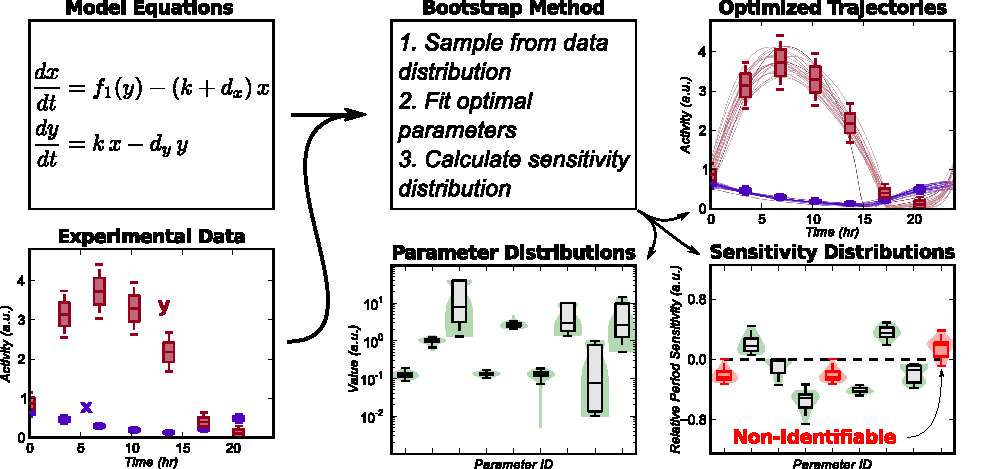
\includegraphics{chap3/figures/fig1.pdf}
  \titlecaption{Parameter estimation and bootstrap methods flowchart}{The demonstrated method calculates confidence intervals in the sensitivity of limit cycle models. An oscillatory model and experimental (or simulated) data are inputs to the bootstrap method. Unique data sets are then used to calculate optimum limit cycle trajectories. The resulting distribution in sensitivities highlight whether a particular response is identifiable (i.e., consistent across the majority of bootstrap trials.)}
  \label{fig:3_1}
\end{figure}

\subsection{Effect of data quality on predictive confidence}

We first analyze the degree to which uncertainty in input data is propagated to uncertainty in output predictions. 
To achieve this, we generate {\itshape in silico} data from a previously published model of circadian rhythms, using relative error $\xi$ to generate normally distributed data ($\sigma_{ij} = \xi \; \hat{x}_{i}(t_j)$) at each of $\cal M$ sampling points. 
As expected, solution trajectories drifted further from the nominal limit cycle for higher values of error, $\xi$, or lower sampling density, $\cal M$, (\fref{fig:3_2}). 
However, the overall shape of the oscillatory profiles remained relatively similar, even for rather high $\xi$ or low $\cal M$.

\begin{figure}[p]
  \centering
  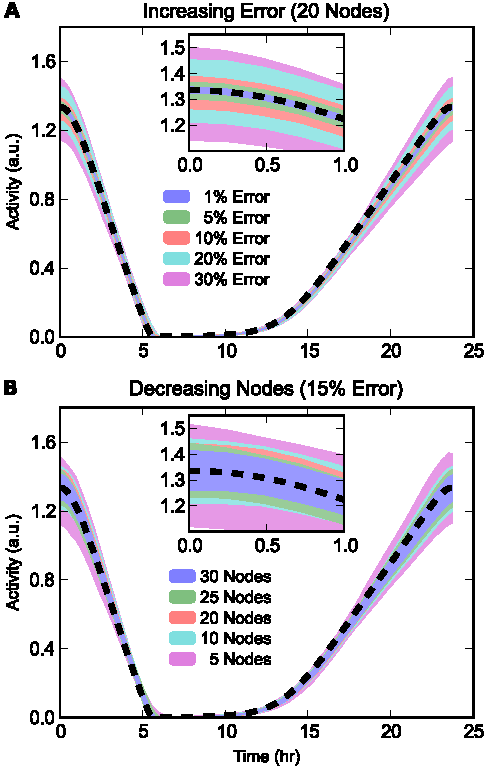
\includegraphics{chap3/figures/fig2.pdf}
  \titlecaption{Time-course profiles of the state trajectories for {\itshape Per mRNA}}{({\bfseries A}) Increasing relative error, $\xi$, with ${\cal M} = 20$. Possible state variable values are shown as shaded regions, obtained by filling between the 5$^\text{th}$ and 95$^\text{th}$ percentile for values at each time for 2000 independent parameter estimations. Increasing $\xi$ results in larger deviations from the original model trajectory, shown as a dashed black line.\\ ({\bfseries B}) Decreasing number of measurement points, $\cal M$, each with $\xi = 0.15$.  Higher $\cal M$ results in trajectories closer to the true trajectory.}
  \label{fig:3_2}
\end{figure}

\Fref{fig:3_3} shows violin plots of the probability distribution for each parameter set and corresponding sensitivity evaluation for increasing $\xi$, while \fref{fig:3_4} shows similar plots for decreasing $\cal M$. 
Interestingly, there is little correlation between the identifiability of a parameter and its corresponding sensitivity value. 
For example, vdP, the maximum degradation rate of Per mRNA, shows a very tight clustering about its nominal parameter value, while the sensitivity of this parameter loses identifiability for even small values of $\xi$. 
Conversely, KdCn, the Michealis-Menten constant associated with the degradation of nuclear CRY, shows large variations in possible parameter values. 
However, the period sensitivity of KdCn, despite lying close to the x-axis, remains identifiable, indicating a robust prediction. 
These results reveal which model responses are constrained by the structure and dynamics of the limit cycle oscillations, and which are dependent on the particular parameterization chosen.

\begin{figure}[p]
  \centering
  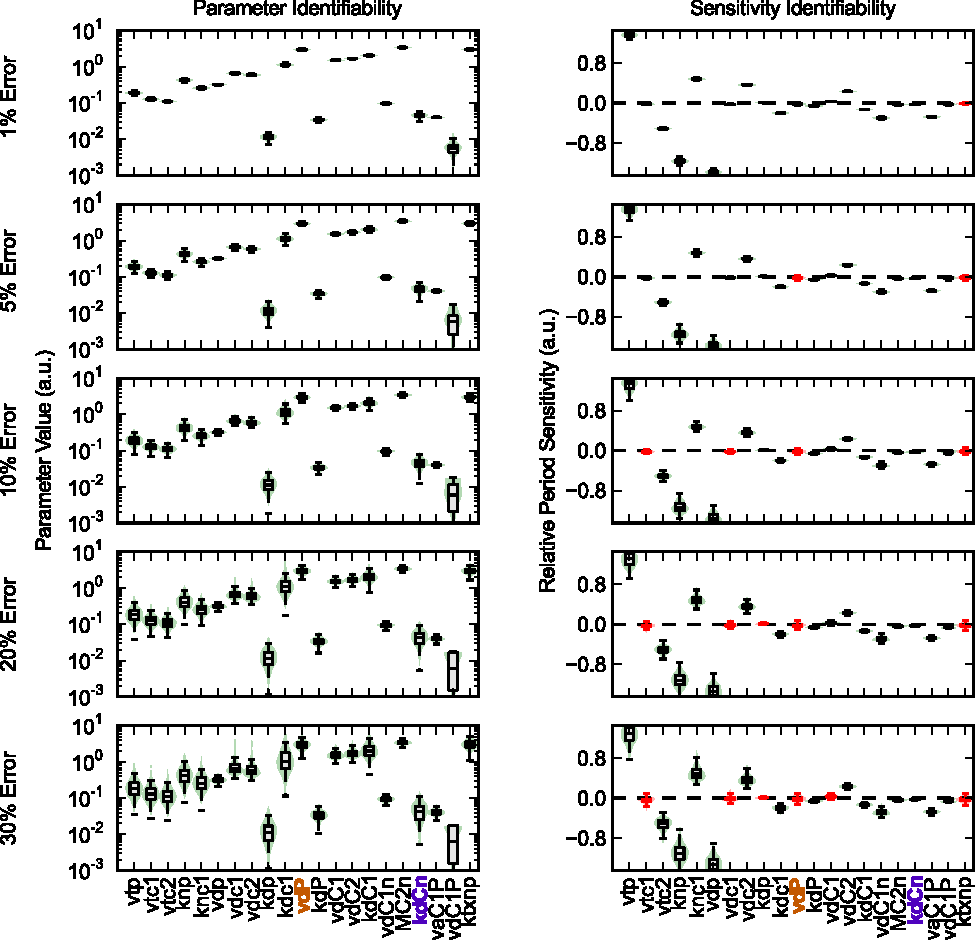
\includegraphics{chap3/figures/fig3.pdf}
  \titlecaption{Parameter and sensitivity identifiability for increasing error}{Increasing $\xi$ results in a corresponding decrease in the confidence of the parameter and sensitivity estimates. Violin plots of the parameter values (left) and relative period sensitivities (right) show the distribution of values from each parameter estimation. In the plots, a box plot is superimposed above a kernel density plot to convey the distribution of values. The whiskers used extend to the most extreme data point within 1.5x the inner quartile range. Sensitivities in which the 5$^\text{th}$ and 95$^\text{th}$ percentile values span the x-axis are deemed non-identifiable (red), as the model's response direction can not be accurately estimated.  Higher $\xi$ also results in wider parameter distributions.}
  \label{fig:3_3}
\end{figure}

\begin{figure}[p]
  \centering
  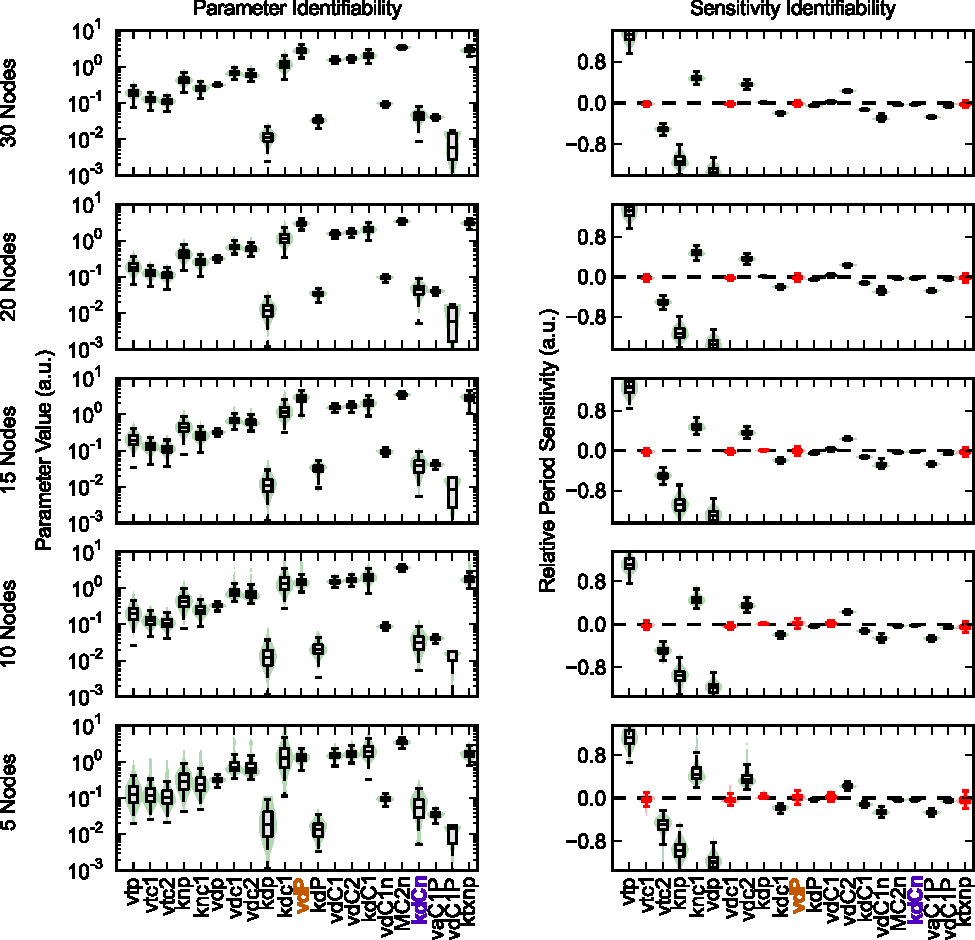
\includegraphics{chap3/figures/fig4.pdf}
  \titlecaption{Effect of high-resolution sampling on identifiability}{ Lower values of $\cal M$ result in less constrained parameter and sensitivity values. Similar to \fref{fig:3_3}, violin plots of the parameters (left) and sensitivities (right) show the distribution from each parameter estimation for decreasing $\cal M$. These results highlight the importance of high-resolution time sampling in generating sensitivity information for oscillatory models.}
  \label{fig:3_4}
\end{figure}

Sensitivities that are experimentally distinguishable from zero are the most important for validation. 
Calculating a typical experimental value for a relative period sensitivity helps to calibrate which sensitivities might be verified experimentally. 
Referring to a recent RNA interference screen, periods changes of approximately 1 hour (~5\%) can be reliably measured using luminescence recordings \cite{Zhang2009}. 
Assuming an increase in the corresponding mRNA degradation parameter value of 50\%, this translates to a relative period sensitivity of ~0.1. 
Thus, many of the identifiable values shown in figures \ref{fig:3_3}-\ref{fig:3_4} fall within the experimentally measurable range. 

\subsection{Application to literature data for model discrimination}
We next apply the method to literature time-course data for core clock components \cite{Lee2001}. 
When modeling a genetic regulatory network, many candidate model equations are often considered. 
We show that a bootstrap uncertainty analysis can also be useful in discriminating between potential model structures based on predictive confidence. 
Here two variations of the same model are fit: The first model (\fref{mod:hirota}) was originally optimized using a genetic algorithm approach, and thus contains a minimal number of parameters to reduce optimization complexity. 
The second model (\fref{mod:hirota2}) considered  contains independent parameters for each rate expression, increasing the number of parameters from 23 to 35. 

\begin{model}[h]
  \centering
  \titlecaption{An expanded parameterization of \fref{mod:hirota}}{These equations have similar reaction stoichiometry to those in table \ref{mod:hirota}, but with more parametric degrees of freedom. This model showed better time-series performance than the more constrained model when fit to time-series data.}

  \begin{align*}
    \frac{d\mathrm{\bf p}}{dt} &= \frac{\mathit{Vm}_{1}}{1 + \mathit{Vm}_{1} \; {\left(\frac{\mathrm{\bf C1N} + \mathrm{\bf C2N} \; \mathit{M}_{1}}{\mathit{Ki}_{1}}\right)}^{3}} - \frac{\mathit{k}_{1} \; \mathrm{\bf p}}{1 + \frac{\mathrm{\bf p}}{\mathit{Km}_{1}}} \\
    \frac{d\mathrm{\bf c1}}{dt} &= \frac{\mathit{Vm}_{2}}{1 + \mathit{Vm}_{2} \; {\left(\frac{\mathrm{\bf C1N} + \mathrm{\bf C2N} \; \mathit{M}_{2}}{\mathit{Ki}_{2}}\right)}^{3}} - \frac{\mathit{k}_{2} \; \mathrm{\bf c1}}{1 + \frac{\mathrm{\bf c1}}{\mathit{Km}_{2}}} \\
    \frac{d\mathrm{\bf c2}}{dt} &= \frac{\mathit{Vm}_{3}}{1 + \mathit{Vm}_{3} \; {\left(\frac{\mathrm{\bf C1N} + \mathrm{\bf C2N} \; \mathit{M}_{3}}{\mathit{Ki}_{3}}\right)}^{3}} - \frac{\mathit{k}_{3} \; \mathrm{\bf c2}}{1 + \frac{\mathrm{\bf c2}}{\mathit{Km}_{3}}} \\
    \frac{d\mathrm{\bf P}}{dt} &= \mathit{k}_{4} \; \mathrm{\bf p} + \mathit{k}_{12} \; \mathrm{\bf C1N} + \mathit{k}_{13} \; \mathrm{\bf C2N} - \frac{\mathit{k}_{7} \; \mathrm{\bf P}}{1 + \frac{\mathrm{\bf P}}{\mathit{Km}_{4}}} - \mathit{k}_{10} \; \mathrm{\bf P} \; \mathrm{\bf C1} - \mathit{k}_{11} \; \mathrm{\bf P} \; \mathrm{\bf C2} \\
    \frac{d\mathrm{\bf C1}}{dt} &= \mathit{k}_{5} \; \mathrm{\bf c1} + \mathit{k}_{12} \; \mathrm{\bf C1N} - \frac{\mathit{k}_{8} \; \mathrm{\bf C1}}{1 + \frac{\mathrm{\bf C1}}{\mathit{Km}_{5}}} - \mathit{k}_{10} \; \mathrm{\bf P} \; \mathrm{\bf C1} \\
    \frac{d\mathrm{\bf C2}}{dt} &= \mathit{k}_{6} \; \mathrm{\bf c2} + \mathit{k}_{13} \; \mathrm{\bf C2N} - \frac{\mathit{k}_{9} \; \mathrm{\bf C2}}{1 + \frac{\mathrm{\bf C2}}{\mathit{Km}_{6}}} - \mathit{k}_{11} \; \mathrm{\bf P} \; \mathrm{\bf C2} \\
    \frac{d\mathrm{\bf C1N}}{dt} &= \mathit{k}_{10} \; \mathrm{\bf P} \; \mathrm{\bf C1} - \mathit{k}_{12} \; \mathrm{\bf C1N} - \frac{\mathit{k}_{14} \; \mathrm{\bf C1N}}{1 + \frac{\mathrm{\bf C1N} + \mathrm{\bf C2N} \; \mathit{M}_{4}}{\mathit{Km}_{7}}} \\
    \frac{d\mathrm{\bf C2N}}{dt} &= \mathit{k}_{11} \; \mathrm{\bf P} \; \mathrm{\bf C2} - \mathit{k}_{13} \; \mathrm{\bf C2N} - \frac{\mathit{k}_{15} \; \mathrm{\bf C2N}}{1 + \frac{\mathrm{\bf C1N} + \mathrm{\bf C2N} \; \mathit{M}_{5}}{\mathit{Km}_{8}}} 
  \end{align*}
  \label{mod:hirota2}
\end{model}


\begin{table}[p]
  \titlecaption{Parameter values for \fref{mod:hirota2}}{Parameters were fit to time-series data via nonlinear programming.}
  \label{tab:parsetopt}
  \vspace{2mm}
  \centering
  \begin{tabular}{cllr} \toprule
           & Parameter        & Description                      & Value  \\ \midrule
    1      & $\mathit{M}_{1}$  & {\itshape Per}/CRY2 activity coefficient    & \num{3.632e+00} \\
    2      & $\mathit{Vm}_{1}$ & {\itshape Per} transcription rate           & \num{9.957e-01} \\
    3      & $\mathit{Ki}_{1}$ & {\itshape Per}/CRY inhibition coefficient   & \num{1.054e-01} \\
    4      & $\mathit{M}_{2}$  & {\itshape Cry1}/CRY2 activity coefficient   & \num{1.000e-03} \\
    5      & $\mathit{Vm}_{2}$ & {\itshape Cry1} transcription rate          & \num{2.262e-01} \\
    6      & $\mathit{Ki}_{2}$ & {\itshape Cry1}/CRY inhibition coefficient  & \num{2.049e-01} \\
    7      & $\mathit{M}_{3}$  & {\itshape Cry2}/CRY2 activity coefficient   & \num{1.000e+01} \\
    8      & $\mathit{Vm}_{3}$ & {\itshape Cry2} transcription rate          & \num{1.850e-01} \\
    9      & $\mathit{Ki}_{3}$ & {\itshape Cry2}/CRY inhibition coefficient  & \num{1.427e-01} \\
    10     & $\mathit{k}_{1}$  & {\itshape Per} degradation rate             & \num{2.920e-01} \\
    11     & $\mathit{Km}_{1}$ & {\itshape Per} degradation self-inhibition  & \num{6.609e-01} \\
    12     & $\mathit{k}_{2}$  & {\itshape Cry1} degradation rate            & \num{1.000e+01} \\
    13     & $\mathit{Km}_{2}$ & {\itshape Cry1} degradation self-inhibition & \num{1.823e-02} \\
    14     & $\mathit{k}_{3}$  & {\itshape Cry2} degradation rate            & \num{4.711e-02} \\
    15     & $\mathit{Km}_{3}$ & {\itshape Cry2} degradation self-inhibition & \num{1.000e+01} \\
    16     & $\mathit{k}_{4}$  & {\itshape Per} translation rate             & \num{1.132e-01} \\
    17     & $\mathit{k}_{5}$  & {\itshape Cry1} translation rate            & \num{3.409e-01} \\
    18     & $\mathit{k}_{6}$  & {\itshape Cry2} translation rate            & \num{1.961e-01} \\
    19     & $\mathit{k}_{7}$  & PER degradation rate             & \num{1.000e+01} \\
    20     & $\mathit{Km}_{4}$ & PER degradation self-inhibition  & \num{1.911e-03} \\
    21     & $\mathit{k}_{8}$  & CRY1 degradation rate            & \num{1.000e+01} \\
    22     & $\mathit{Km}_{5}$ & CRY1 degradation self-inhibition & \num{2.077e-02} \\
    23     & $\mathit{k}_{9}$  & CRY2 degradation rate            & \num{1.000e+01} \\
    24     & $\mathit{Km}_{6}$ & CRY2 degradation self-inhibition & \num{1.180e-02} \\
    25     & $\mathit{k}_{10}$ & C1N association rate             & \num{5.022e-01} \\
    26     & $\mathit{k}_{11}$ & C2N association rate             & \num{1.035e+00} \\
    27     & $\mathit{k}_{12}$ & C1N dissociation rate            & \num{1.000e-03} \\
    28     & $\mathit{k}_{13}$ & C2N dissociation rate            & \num{2.070e-01} \\
    29     & $\mathit{M}_{4}$  & CRY1n/CRY2n activity coefficient & \num{1.000e+01} \\
    30     & $\mathit{k}_{14}$ & CRY1N degradation rate           & \num{1.000e+01} \\
    31     & $\mathit{Km}_{7}$ & CRY1n degradation inhibition     & \num{5.206e-03} \\
    32     & $\mathit{M}_{5}$  & CRY2n/CRY2n activity coefficient & \num{1.000e+01} \\
    33     & $\mathit{k}_{15}$ & CRY2n degradation rate           & \num{1.000e+01} \\
    34     & $\mathit{Km}_{8}$ & CRY2n degradation inhibition     & \num{1.829e-02} \\ \bottomrule
    \hline
  \end{tabular}
\end{table}

\begin{figure}[p]
  \centering
  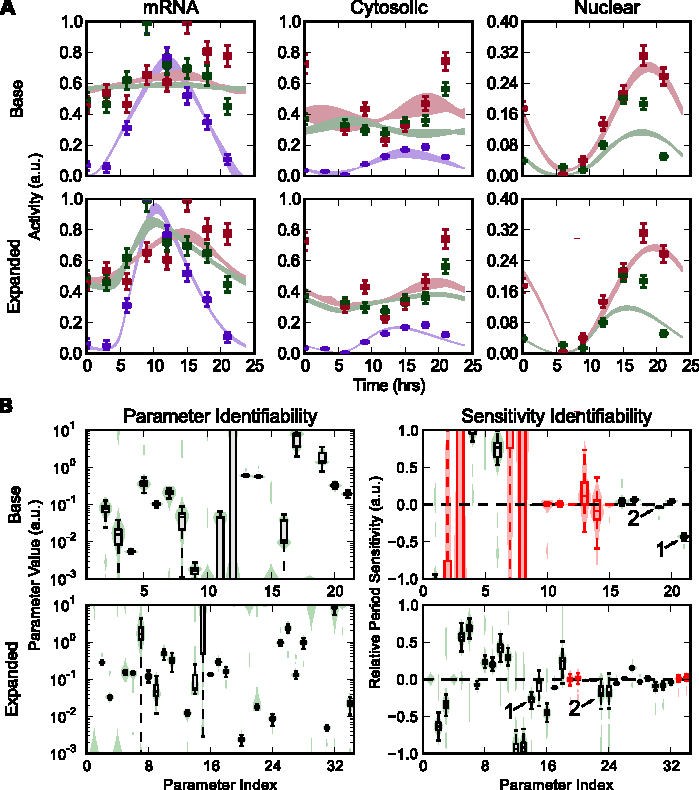
\includegraphics{chap3/figures/fig5.pdf}
  \titlecaption{Identifiability comparison of two model structures}{ ({\bfseries A}) Bootstrap parameter estimations on two model structures using literature time-series data with estimated errors (box plots). Resulting regions of model trajectories are shaded between the 5$^\text{th}$ and 95$^\text{th}$ percentile.  {\itshape Per} species are shown in purple, {\itshape Cry1} in red, and {\itshape Cry2} in green. While both models were able to approximately reproduce the same dynamic response, the expanded model was better able to capture differences between the {\itshape Cry1} and {\itshape Cry2} profiles. ({\bfseries B}) Parameter and sensitivity identifiability for the base and expanded models.  Violin plots show the parameter and sensitivity distributions, with unidentifiable sensitivities (90\% confidence level) highlighted in red.  Despite containing more parameters, the expanded model shows better parameter identifiability and higher confidence in its predicted sensitivities. The PER translation rate (1) and PER-CRY association rate (2) sensitivities are consistent across model equations and are highlighted.}
  \label{fig:3_5}
\end{figure}

The literature data used consisted of 7-8 concentration time points across a 24 hour period. 
Confidence intervals in the data were not available, so an optimistic 3\% relative and 0.5\% absolute error was assumed for each data point ($\sigma_{ij} = 0.03\;\hat{x}_{i}(t_j) + 0.005\;\max(\hat{x}_i)$). 
\Fref{fig:3_5}A shows the resulting time-series profiles for bootstrap estimations of each model. 
While additional kinetic parameters are typically thought to lower the predictive confidence of a model (the `curse of dimensionality'), the expanded model is able to better capture the oscillatory profiles with lower variability between solutions. 
Parameter and sensitivity distributions, figure \ref{fig:3_5}B, similarly show how the expanded model parameterization is able to generate more confident predictions in model response. 
Since the resulting sensitivity identifiability for both models was relatively poor, we highlight sensitivities which pass a 90\% confidence level threshold. 
These results thus indicate higher-resolution data on circadian components would help in conferring confidence to model predictions.

Two sensitivities, the PER translation rate (figure \ref{fig:3_5}B, 1) and the PER-CRY association rate (2), had high confidence and consistent direction in both the base and expanded parameterization - suggesting that the predicted values are robust to slight changes in both parameter value and model structure. 
Since a biological system can be modeled using many different combinations of kinetic assumptions, such a technique will likely prove useful in finding consistent predictions which are robust to slight differences in model equations.

\Fref{fig:3_6} compares optimal fits for both the base and expanded models to the originally published parameter set \cite{Hirota2012}. 
Since the original cost function was concerned mostly with optimizing stoichiometric and knockout data, the refitted models are able to much more accurately represent the time-series dynamics. 

\begin{figure}[p]
  \centering
  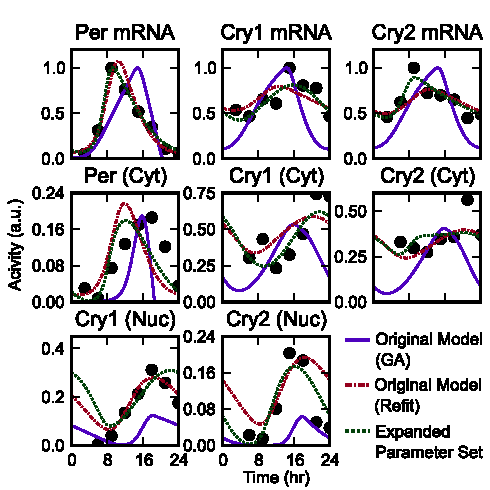
\includegraphics{chap3/figures/fig6.pdf}
  \titlecaption{Time-series dynamics of fitted models}{Model trajectories for each of the considered models. The original model (purple) shows the time series dynamics for the previously published parameter set, used in Figures 1-4. In these plots, the original model's period and amplitudes were rescaled to best match the experimental data, shown in black (without changing the dynamic profiles). The refitted model (red, dashed) was generated by optimizing the dynamic profile to time series data using the parameter estimation routine described in Supplemental Text 1. The expanded model (green, dashed) consists of a similar network structure, but with independent kinetic parameters for each rate expression (see Supplemental Text 2). These plots show that parameter optimization through nonlinear programming is able to more accurately fit gene and protein expression profiles.}
  \label{fig:3_6}
\end{figure}

\section{Discussion}
Increasingly, mathematical models are being used to study biological systems where traditional experiments would prove infeasible. 
 For example, in the search for drug targets, thousands of possible combinatorial perturbations can be quickly scanned for therapeutic effects using {\itshape in silico} modeling. 
This is especially useful in oscillatory systems with long periods, such as circadian rhythms, where a perturbed {\itshape in vitro} or {\itshape in vivo} system must be measured for multiple days before changes can be reliably determined.
 
However, since errors in model responses can arise from either incorrect structure or measurement noise, our confidence in {\itshape in silico} predictions is limited. 
Here we have developed a bootstrap approach suitable for periodic systems, and extended it to include uncertainty in predicted responses. 
With this method, errors due to local parameter effects can be identified, even in models with complicated dynamics. 
Furthermore, by considering multiple variations in model assumptions, we have demonstrated that more trustworthy model predictions can be found.

Since this method takes advantage of time-series data to generate a strong initial guess for an otherwise difficult parameter estimation, it requires high-resolution data on the concentrations of all species in the model. 
In many biological systems, such data is only available for the activity levels of certain well-studied species. 
However, the continued development of high-throughput genomic and proteomic techniques promise to deliver time-series data for a much larger network of components. 
With expanding datasets, these methods will likely prove useful for the quantitative evaluation of uncertainty in larger biological models.

In the following chapter, I apply this method to several existing circadian models in order find conserved predictions across different model kinetics and parameterizations. 
Such an approach allows us to further differentiate between the actions of two seemingly similar small molecule perturbations. 
